\section{DroneCharge}
\subsection{Vision}
We envisioned DroneCharge as a framework to be used by drone application developers to easily achieve task-execution using swarms of drones, and as such needed to fit any and all suitable drones. As all drones have their own native APIs for control, this meant that a driver-oriented architecture had to be utilized. While the drivers provided us with means of controlling the drone, we also needed a way of hooking into the tasks performed by the drones in order to seamlessly exchange drones when required. This was done by having developers define tasks in terms of a series of subtasks, and to have our framework execute those tasks in the right order. That enabled us to hook into the execution of a task and to exchange drones when a recharge was needed. As such, the envisioned system would have the following functionality:

\begin{itemize}
    \itemsep0em
	\item Automatic recharging of battery-depleted drones
	\item Task pausing and resumption
	\item Drone swapping between tasks
	\item Simplified usage of heterogenous drones for task execution
\end{itemize}

\subsection{Architecture}
Our overall architecture is depicted in Figure \ref{fig:architecturefig}. The most interesting concepts are the ideas of drone, task and environment. A task is performed in an environment that has a number of drones at its disposal, all of which are configured by the individual developer. As a developer, you would implement drivers for your specific drone that inherits from the \textit{Drone} class, and either utilize the built-in tasks or create your own extension of the \textit{Task} class. A drone instance representing each physical drone is then added to the environment along with their respective charging locations, as well as any number of tasks to be performed.

\begin{figure}[h]
\centering
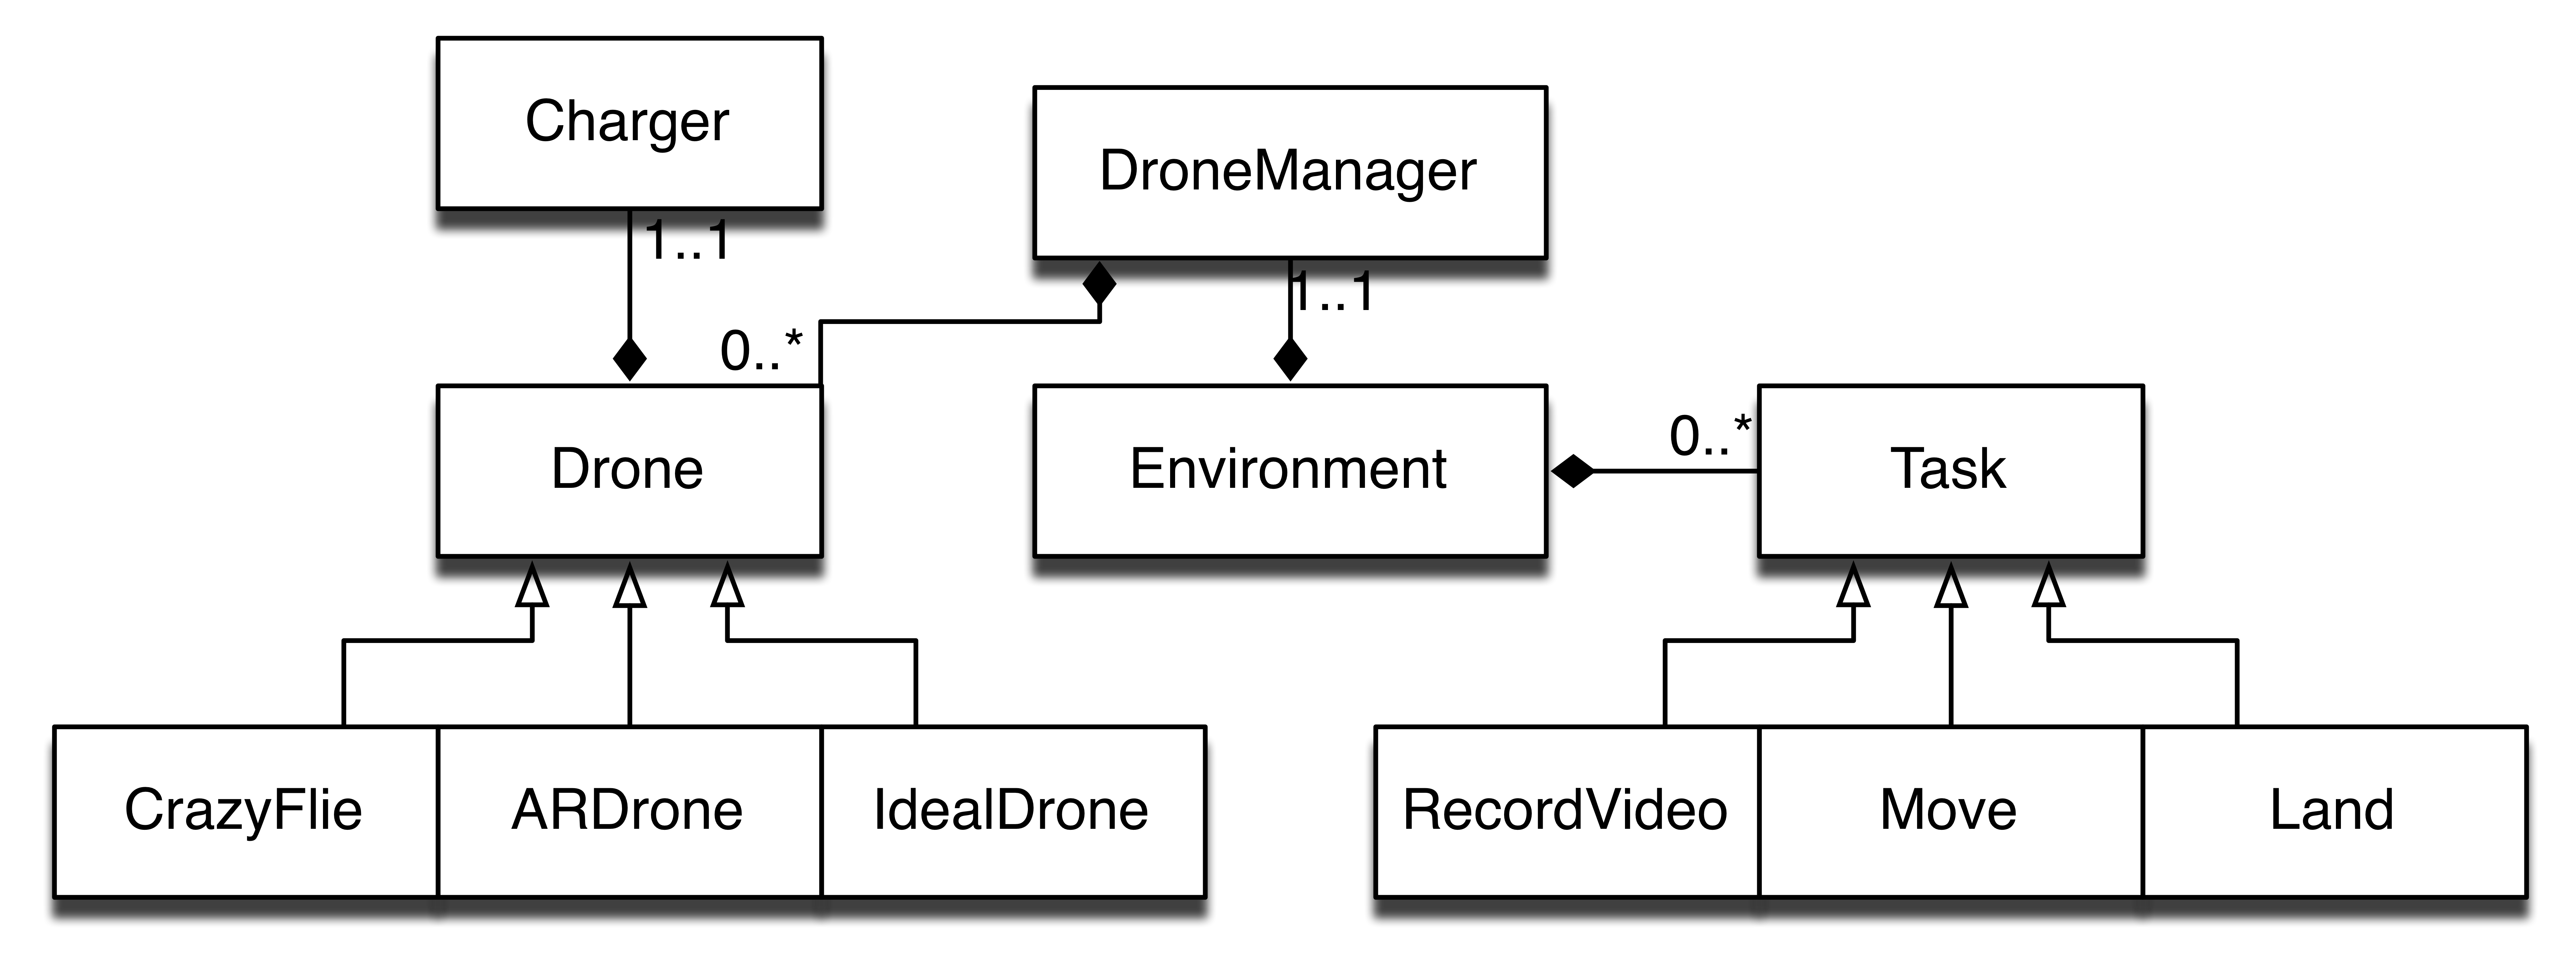
\includegraphics[width=\columnwidth]{images/dronechargearchitecture.png}
\caption{DroneCharge architecture}
\label{fig:architecturefig}
\end{figure}

\subsection{Environment}
The notion of environment provides an abstraction over the physical environment. We introduced the idea of an abstract coordinate system, which lets the implementers use any unit or orientation (GPS coordinates, meters, pixels, or completely abstract units) as long as they stick to the same unit throughout the drone driver and task definitions. Because it is the drone driver, that is responsible for both supplying and consuming the current and target positions of the drone, the abstract unit system does not limit the framework to any particular assumptions about the positions.

\subsection{Drivers}
Drivers are, as is the definition, a way for the system to interact with the hardware devices connected to it without knowing the hardware specifications at compile-time. In our case, those hardware devices are drones and their locationing system. Any developer using DroneCharge must implement a class extending from the Drone-class that implements neccesary features such as movement as well as battery- and location-queries. These are called drone-drivers. Whether a drone has positioning built-in or if it uses a tertiary system such as tracking with a Microsoft Kinect is irrelevant, as long as the drone-driver has the ability to obtain its position. A drone driver has to be able to identify the position of its assigned physical drone with a specified precision and perform movement to a target position set by the framework.

\subsection{Tasks}
Instances of the \textit{Task} define how individual steps of a task are performed. They contain a list of capabilities required to perform the task such as movement or video-recording, as well as instructions on how to perform the task. DroneCharge comes with a limited number of built-in tasks such as movement and landing, but any task can be performed by extending the task class and explicitly performing the task through the commands defined in the drone-drivers. The framework will only assign drones to perform the task if they meet the requirements for it, so you are guaranteed to have the right type of drone as long as your task and required capabilities are aligned. As an example, a custom driver for a drone with a video camera attached to it could implement a function called \textit{RecordVideo} as well as contain the capability \textit{recordvideo}. You could then define a task whose execution consisted of turning on a video camera. By specifying \textit{recordvideo} as a required capability of the task, the framework would not perform the task until a drone with said capability was available. The framework does not make any assumptions about the tasks, it is the task instance, that is responsible of deciding what to perform and when it is complete. This way a user of the framework can implement both, the task and the drone driver and so the task will know how to perform specific functionality with a particular drone.

\subsubsection{The Task Tree}
By allowing tasks to be added to other tasks, we obtained a tree-structure view of tasks which enabled us to do a depth-first search traversel of tasks, and in that way achieve a sound logical structuring of tasks and subtasks. An example of such a tree is depicted in Figure \ref{fig:tasktree}. The tree is traversed in such a way that only leaf-node-tasks are actually performed. This enabled developers to logically split their tasks into subtrees however they saw fit and gave us increased flexibility. When a drone was to take over a task, a replacement-task could easily be inserted in that tree that moved the drone to the position of the depleted drone and performed other actions such as copying the state of the previous drone, turning on sensors etc.

\begin{figure}[h]
\begin{center}
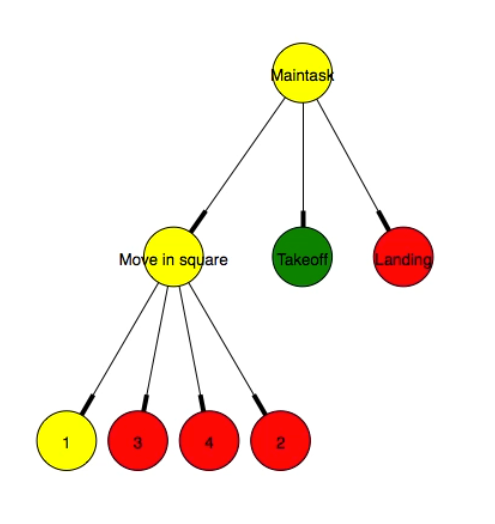
\includegraphics[height=7cm]{images/task-graph.png}%
\caption{The Task Tree -- NB: Nodes are \textit{not} ordered in a DFS-like manner as is the case internally}
\label{fig:tasktree}
\end{center}
\end{figure}

\subsection{Assumptions and requirements}
When using the DroneCharge framework, developers had to be aware of the assumptions and requirements made in terms of the capabilities and implementation of the drivers and the drones themselves.

For the drone drivers, we assumed that a drone or its driver could report its battery level in a linear fashion. That is, the battery could not be reported as full until the battery was depleted as was the case with some drones such as the Crazyflie. Furthermore, there had to be some way to obtain the position of the drone in relative or absolute terms. A developer also had to define at what battery level the drone was considered to be low on battery. It was also required that a charger was available for each individual drone.

In terms of defining tasks, we made the requirement that any single leaf-node in the tree could not require more battery to perform than was considered to be the low battery limit. That is, if the drone was considered to be at low battery when it reached 10\%, all individual subtasks had to require no more than 10\% power to perform. Finally, the point of operation that was the farthest from the charging station could not require more than the low battery level to move the drone from back to the charger.

Additionally, it was noted that a drone partaking in the execution of a task had to have all capabilities  needed to perform all subtasks in the task tree in which the current subtask is located. This is upheld by the framework itself, as it will not choose drones lacking the capabilities. This ensured that we would not have to exchange drones due to capabilities but only due to battery levels.
